\chapter{Ist-Analyse}

Nachdem im letzten Kapitel ein grober Überblick über die bestehende Problemstellung, sowie den geplanten Lösungsweg gegeben wurde, folgt ein kurzer Einblick in die bestehenden Technologien um die Vorteile modernerer Technologien zu beleuchten. 

\section{JBoss (Microprofile) \checkmark}

% \begin{itemize}
%   \item aktuelle Architektur beschreiben
%   \item Hinweis darauf geben, dass Prototyp in der Thesis vereinfacht mit Spring dargestellt wird
%   \item jetzt ja fiktiv SpringBoot, hier rein technischer Ist-Stand, Systemarchitektur….
% \end{itemize}


\begin{figure}[b!]
	\centering
	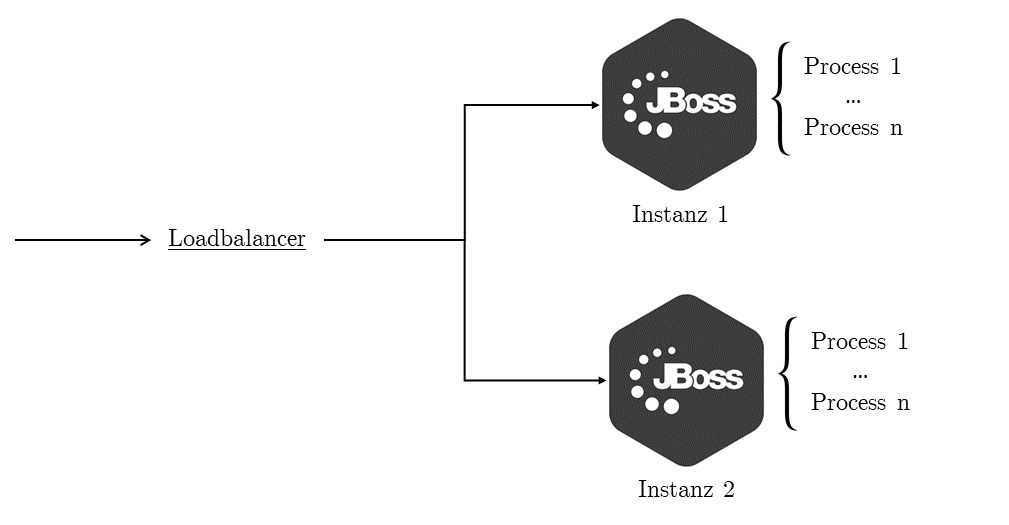
\includegraphics[width=.7\linewidth]{kapitel/ist-analyse/_img/jbossOverview}
	\caption[JBoss Systemaufbau]{JBoss Systemaufbau}
	\label{fig:jbossArch}
\end{figure}


Die aktuelle Verarbeitung von Payments innerhalb der Anwendung läuft in Produktion auf vier Instanzen des kommerziellen Applikation-Servers "\emph{JBoss}". Im Development wird hierbei eine Open-Source Variante namens "\emph{Wildfly}" verwendet. In diesen Application Servern werden .war Dateien deployed, welche den ausführbaren Code der Anwendung beinhalten. Der Application Server bietet dem Backend der Anwendung eine Laufzeitumgebung, in der die Anwendung ausgeführt werden kann. JBoss bietet nun standardisierte Schnittstellen nach dem jeweils festgelegten Java-Enterprise-Standard, um zum Beispiel die Kommunikation mit der Außenwelt zu ermöglichen oder der Anwendung eine Persistenzschicht zur Verfügung zu stellen. Außerdem laufen die Instanzen im \emph{Microprofile} Modus, der es möglich macht, dass bestimmte Konfigurationsparameter ausgelagert werden. So können Applikationen auf unterschiedlichen Systemen deployed werden, ohne komplett neu gebaut zu werden (siehe \cite{microprofile}). Um eine gleichmäßige Aufteilung der Last zu gewährleisten, teilt ein sogenannter "\emph{Load Balancer}" die eingehenden Nachrichten den entsprechenden Instanzen zu (siehe Abbildung \ref{fig:jbossArch}). Jede der vorhandenen Instanzen besitzt eine minimale sowie maximale Anzahl an parallel ausführbaren Prozessen. Diese Angaben werden auch "\emph{max. / min. Poolsize}" genannt. Eine minimale Poolsize muss gegeben sein, um sicherzustellen, dass eine gewisse Grundlast, falls nötig, sofort bearbeitet werden kann, daher darf diese Anzahl auch nicht Null betragen. Die maximale Poolsize stellt sicher, dass es zu keiner Überlastung des Systems kommt. Wenn eine Instanz bereits mit der maximale Anzahl an Prozessen arbeitet, wird dies dem Loadbalancer signalisiert und welcher wiederum der entsprechenden Komponente in diesem Zeitraum keine weiteren Nachrichten mehr zuteilt. Um zu gewährleisten, dass die Nachrichten nicht verloren gehen, werden sie in eine Warteschlange ("\emph{Request Queue}") geschrieben, welche lediglich dazu gedacht ist, den Overhead abzuspeichern. Wie die Daten im Detail verarbeitet werden, ist für die weitere Betrachtung irrelevant und wird daher nicht weiter erläutert. Eine vereinfachte Implementierung wird im späteren Prototypen dennoch vorhanden sein. Die dazugehörige Beschreibung befindet sich in Abschnitt \ref{ss:fiktiverWorkflow}.


\section{Probleme \checkmark}

% https://easy-software.com/de/newsroom/microservices-vs-monolith/
% \todo{Quelle einfügen}


% \begin{itemize}
%   \item Probleme mit aktuellem System (Stichwort Deployment, Wartbarkeit)
%   \item Prof. hat extra darauf hingewiesen, dass es nicht nur um die Vorteile der Cloud gehen soll
%   \item „Erwartete Probleme in einer Cloud Umgebung“ à aktuell „..starre Hardware und Software- Skalierung…“ unerwartete lastspitzen könnten zu problemen führen, wenn sie die erwartete und verfügbare obergrenze an kapazität übersteigt und wie oben gesagt ineffiziente nutzung von kapital….nochmal mit anderen worten aus 
%   \item  1.2 à die auflistung der probleme hier, müssen dann in der zusammenfassung wieder auftauchen und abgehakt werden! Die wollen wir ja auch lösen…
% \end{itemize}


Bezüglich der Systemarchitektur einer klassischen Java-Enterprise Anwendung handelt es sich in der Regel um eine monolithische Struktur. Die ausführbare Anwendung wird mit Hilfe von einer einzigen Codebase entwickelt, gebaut und deployed. Dem gegenüber steht die \emph{service-basiert} Designstruktur, dabei handelt es sich um eine mittels Containern ermöglichten Umgebung. Weshalb monolithische Systeme den heutigen Anforderungen in manchen Aspekten nicht mehr genügen und inwiefern eine service-basierte Struktur hierbei Abhilfe schafft wird im folgenden näher erläutert \cite[Seite~42 ff.]{continuous-delivery}.

\subsection{Skalierte Entwicklung \checkmark}
Wenn viele Entwickler an derselben Anwendung arbeiten, muss jeder einzelne zumindest ein grundlegendes Verständnis der gesamten Codebase besitzen. Außerdem kommt es während der Entwicklungszeit zwangsweise zu einer Reihe von Mergekonflikten. Mit den richtigen Designprinzipien bezüglich der losen Kopplung der einzelnen Komponenten sowie der Modularisierung des Systems, sollte dies zwar eigentlich umgangen werden können, in der Realität entwickelt sich ein solches System allerdings ständig weiter. Da das System diese Prinzipien allerdings nicht explizit erzwingt, werden diese Prinzipien häufig mit der Zeit vernachlässigt. Funktionalität aus dem Modul zu extrahieren und in eigenständige Services auszulagern führt hierbei zu einem effizienteren Workflow. Insbesondere hinsichtlich der Arbeitsaufteilung ermöglicht der service-basierte Aufbau die Implementierung klarer Schnittstellen, wodurch viele Entwickler parallel arbeiten können.


\subsection{Unabhängiges Deployment \checkmark}
Eine monolithische Applikation wird mit Hilfe eines einzelnen Artifacts deployed. Dies stellt insbesondere dann ein Problem dar, wenn neue Funktionalität implementiert wird oder einzelne Teile der Applikation häufiger verändert werden als andere. Bei allen genannten Szenarien muss stets die gesamte Applikation neu deployed werden obwohl die Veränderungen nur einzelne Komponenten der Anwendung betreffen. Bei einem stark gekoppelten System muss jede neu hinzugefügte Funktionalität verstärkt getestet werden, da es möglicherweise Abhängigkeiten zwischen Komponenten gibt, die auf den ersten Blick als solche eventuell gar nicht erkennbar sind. Der Service-basierte Ansatz bietet hier Abhilfe, da es möglich ist ausschließlich dedizierte Teile des Systems (neu) zu deployen beziehungsweise nur noch diejenigen Komponenten testen zu müssen, welche überhaupt verändert wurden, ohne dabei Risiken einzugehen. 


\subsection{Skalierung in Produktion \checkmark}
Eine Skalierung ist mit monolithischen Strukturen nur dadurch möglich, den ausführbare Code auf zusätzlichen Servern zu deployen, dies wird auch \emph{horizontale Skalierung genannt}. Jede dieser Kopien nutzt die gleiche Resourcenanzahl, was es zu einem ineffizienten Design macht, da sie sich nicht dynamisch der gegebenen Last anpassen. Tatsächlich ist ein es jedoch ein viel größeres Problem, wenn ein bereits aufgeteiltes System an seine Kapazitätsgrenze stößt, denn Java-Anwendungen besitzen eine relativ lange Initialisierungsphase. Um den heutigen Anforderungen der dynamischen Skalierung gerecht zu werden, werden Resourcen auf Abruf gebraucht. Die Systeme sollen so schnell wie möglich verfügbar sein. Außerdem ist es bei monolithischen Systemen ausgeschlossen nur die betreffenden Komponenten des Systems zu skalieren, die durch eine erhöhte Last überhaupt betroffen sind.


% Mit der monolithischen Struktur des aktuellen Systems kommt es im Laufe der Zeit zu unterschiedlichen Problemen. Über die Zeit werden Komponenten immer weiter verstrickt, sodass es in einem solchen System auch nach Personalwechsel nicht einfacher wird den Überblick über die gesamt Applikation zu behalten. Dies führt zu fehleranfälligerem Code, welcher sich wiederum negativ auf das Kapital einer Firma niederschlägt. Diese Fehler führen in einem monolithischen System zu einem großräumigen Ausfall der gesamten Applikation, da es keine klare Abgrenzung der einzelnen Komponenten gibt. 

% Außerdem laufen die Application Server auf Servern, die (wenn überaupt) eine sehr dünne Abstraktionsschicht bieten ("\emph{starrer Hardware}"). Es ist nicht möglich diese schnell und flexibel zu ersetzen, falls es zu Fehlern in der Produktionsphase kommen sollte. Application Server bringen einen großen Konfigurationsaufwand mit sich, der sich schlecht automatisieren lässt. Man braucht geschultes Fachpersonal um ein solches System zum Laufen zu bekommen.

